Here is a sentence, and you can see a nice picture in Figure \ref{fig:brayford}.

\begin{figure}[h]
    \centering
    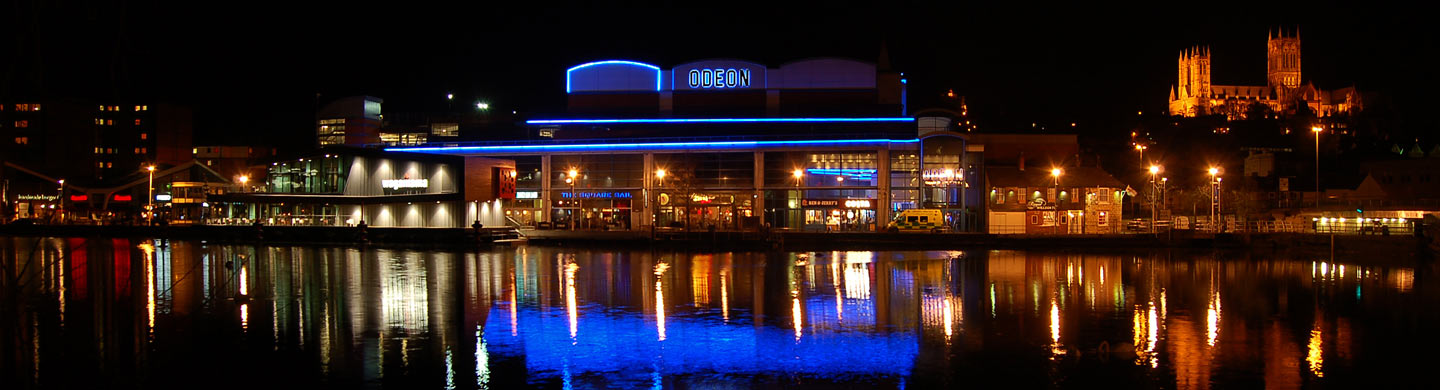
\includegraphics[width=\textwidth]{figures/brayford.jpg}
    \caption{A picture of the Brayford from Google Images.}
    \label{fig:brayford}
\end{figure}

Also, a table can be found in Table \ref{tbl:example-table}. You should use a \LaTeX~table generator like \url{https://www.tablesgenerator.com/} if you want to make your life easier.

\begin{table}[h]
    \caption{Here is a table. The caption goes above like this.}
    \centering
    \begin{tabular}{l|l|c}
        First name & Last name & Age \\
        \hline\hline
        Bob & Bobbington & 24 \\
        Benth & Wavies & 49 \\
        Joe & Bloggs & 37 \\
        Billy & Bob & 10 \\

    \end{tabular}
    \label{tbl:example-table}
\end{table}

This section will cover a number of aspects of your project where appropriate. Not all projects will require every section though.The key thing is that you demonstrate critical awareness of all of the processes that you have employed in your work and that for all sections needed in your report you are presenting a justification for the methods you adopted and not just presenting a list of methods.

\section{Project Management}
Some awareness of project management should be demonstrated in all projects. This section should outline the nature of your project and the specific characteristics that need to be considered in determining  what project management methodology you should use. You should identify the specific demands of your project in terms of project management and support your rationale for the selection of a methodology with appropriate and recent academic references. Questions which may be relevant here are:
\begin{enumerate}
    \item What are the guiding principles and processes in managing your project?
    \item What project management methods may be useful for this project?
    \item How can you exploit their advantages for your project and mitigate their drawbacks?
\end{enumerate}

\section{Software Development}
There should be a methodological analysis of software development approaches used in your project. It is important to note that what is NOT required here is a pedestrian account of popular software development methodologies or a simplistic review of their strengths and weaknesses. 

Where relevant, you should give serious thought to the proper design of research and requirements capture approaches. This may include surveys, questionnaires and interviews. 

\section{Toolsets and Machine Environments}
Toolsets refer to both software development and to project management, so the coverage should address both. This section will outline the tools for software development and project management process; it will make appropriate comparisons between tools available and argue for the most appropriate selection based on metrics, possibly a matrix diagram and other criteria.

DO NOT justify the grounds for using specific toolsets and environments simply because you know them well or have developed skills already. 

\section{Research Methods}
You should investigate the types of research methods necessary to validly answer the research questions that your project addresses. You should cite relevant sources to justify your choices.

